\section{Metodo di Hess-Smith}

Si vuole calcolare la corrente incomprimibile irrotazionale bidimensionale attorno a un profilo aerodinamico, utilizzando il principio di sovrapposizione delle cause e degli effetti per ottenere il campo di moto attorno al profilo come somma della velocità uniforme e della velocità di alcune soluzioni elementari dell'equazione di Laplace per il potenziale, come sorgenti e vortici.\newline
Per motivi di accuratezza del metodo, non vengono utilizzate singolarità puntiformi (come sorgenti o vortici puntiformi), ma vengono utilizzate delle singolarità distribuite su i segmenti che descrivono la geometria discretizzata del profilo.

\subsection{Descrizione della geometria}
Il profilo aerodinamico viene suddiviso da $N+1$ punti in $N$ elementi (o pannelli).
Per ogni elemento, vengono definite alcune grandezze geometriche: la lunghezza $\ell_k$, i versori normali e tangenti $\bm{\hat{n}}_k$, $\bm{\hat{t}}_k$, i punti estremi del pannello $\bm{x}^1_k$, $\bm{x}^2_k$ (che verrano utilizzate per calcolare le velocità indotte dai pannelli) e il punto di controllo coincidente con il centro del pannello $\bm{x}^c_k$ (che sarà il punto nel quale verranno imposte le condizioni al contorno).

\begin{tcolorbox}
La funzione \texttt{build\_geometry()} legge i dati di un profilo NACA, le sue dimensioni e posizione nello spazio e resitituisce la struttura \texttt{elems} che contiene le informazioni sui pannelli, insieme alle matrici che contengono coordinate dei punti \texttt{rr}, la connettività nodi-elementi \texttt{ee}, l'indice dei pannelli al bordo di uscita \texttt{ii\_te}, il numero \texttt{nelems} di elementi e \texttt{npoints} di punti. \newline
\texttt{[ rr, ee, ii\_te, elems, nelems, npoints ] = build\_geometry( airfoil) }
\end{tcolorbox}

\subsection{Principio di sovrapposizione delle cause e degli effetti: campo di velocità}
Vengono utilizzate i seguenti campi di velocità irrotazionali:
\begin{itemize}
 \item corrente uniforme $\bm{U}_{\infty}$;
 \item $N$ distribuzioni costanti di sorgenti su ogni pannello, di intensità $\sigma_k$, $k=1:N$; 
 \item $N$ distribuzioni costanti di vortici su ogni pannello, di intensità $\gamma_k$, $k=1:N$.
\end{itemize}
La velocità indotta nel punto $\bm{x}$ da una distribuzione costante di sorgente su un pannello di intensità $\sigma_k$ è
\begin{equation}
  \bm{u}^s_k(\bm{x}) = \left[
  - \dfrac{1}{2\pi} \ln \dfrac{|\bm{r}_2|}{|\bm{r}_1|} \bm{\hat{t}}_k 
  + \dfrac{1}{2\pi} \beta \bm{\hat{n}}_k \right] \sigma_k =
  \bm{u}^{s,1}_k(\bm{x}) \sigma_k \ ,
\end{equation}
essendo $\bm{\hat{t}}_k$, $\bm{\hat{n}}_k$ i versori tangente e normale\footnote{
    Per ottenere le componenti della velocità nel sistema globale, è necessario esprimere i versori $\bm{\hat{t}}_k$, $\bm{\hat{n}}_k$ nel sistema di riferimento globale formato dai versori $\bm{\hat{x}}$, $\bm{\hat{y}}$. La legge di trasformazione dei vettori delle basi si ottiene proiettando i vettori della base locale nella base globale,
    \begin{equation}
       \bm{\hat{t}}_k =( \bm{\hat{t}}_k \cdot \bm{\hat{x}}) \bm{\hat{x}} + 
                       ( \bm{\hat{t}}_k \cdot \bm{\hat{y}}) \bm{\hat{y}} \qquad , \qquad 
       \bm{\hat{n}}_k =( \bm{\hat{n}}_k \cdot \bm{\hat{x}}) \bm{\hat{x}} + 
                       ( \bm{\hat{n}}_k \cdot \bm{\hat{y}}) \bm{\hat{y}} 
    \end{equation}
 e la legge di trasformazione delle componenti si ottiene come
    \begin{equation} \begin{aligned}
      \bm{u} = u_{k,t} \bm{\hat{t}}_k +  u_{k,n} \bm{\hat{t}}_n =
        ( t_{k,x} u_{k,t} + n_{k,x} u_{k,n} ) \bm{\hat{x}} + 
        ( t_{k,y} u_{k,t} + n_{k,y} u_{k,n} ) \bm{\hat{y}} = 
        u_x \bm{\hat{x}} + 
        u_y \bm{\hat{y}} \ , 
    \end{aligned} \end{equation}
  o in forma matriciale
  \begin{equation}
      \left[ \begin{array}{c} u_x \\ u_y \end{array} \right] =
      \left[ \begin{array}{cc} t_{k,x} & n_{k,x} \\
                               t_{k,y} & n_{k,y} \end{array} \right]
      \left[ \begin{array}{c} u_{k,t} \\ u_{k,n} \end{array} \right] \  .
  \end{equation}
}
al $k$-esimo pannello, i vettori $\bm{r}_i = \bm{x} - \bm{x}^i_k$, $i = 1:2$ e $\beta$ l'angolo compreso tra il vettore $\bm{r}_1$ e il vettore $\bm{r}_2$, positivo se si deve ruotare il vettore $\bm{r}_1$ in senso antiorario per farlo coincidere con $\bm{r}_2$.
Infine é stata espressa la velocità indotta dalla sorgente di intensità $\sigma_k$ come prodotto della velocità indotta da una sorgente unitaria $\bm{u}^{s,1}_k$ e dell'intensità $\sigma_k$. \newline
Allo stesso modo, si può scrivere la velocità indotta da una distribuzione di vortici come
\begin{equation}
 \bm{u}^v_k(\bm{x}) = \bm{u}^{v,1}_k(\bm{x}) \gamma_k \ .
\end{equation}
Il campo di velocità risultante dalla sovrapposizione della corrente uniforme e delle singolarità introdotte è
\begin{equation}
 \bm{u}(\bm{x}) = \bm{U}_{\infty}
  + \displaystyle\sum_{k=1}^{N}\bm{u}^{s,1}_k(\bm{x}) \sigma_k 
  + \displaystyle\sum_{k=1}^{N}\bm{u}^{v,1}_k(\bm{x}) \gamma_k \ .
\end{equation}
Questa espressione del campo di velocità contiene $2\,N$ incognite, le intensità delle sorgenti $\sigma_k$ e dei vortici $\gamma_k$, $k=1:N$.
\begin{tcolorbox}
Le funzioni
\begin{verbatim}
   v = compute_velocity_source( elems_k , rr_i )
   v = compute_velocity_vortex( elems_k , rr_i )
\end{verbatim}
calcolano la velocità \texttt{v} nel punto \texttt{rr\_i} indotta da singolarità di intensità unitaria distribuita sull'elemento \texttt{elems\_k}. Il vettore colonna  \texttt{v} contiene le componenti $x$ e $y$ della velocità, nel sistema di riferimento globale.
\end{tcolorbox}

\subsection{Metodo di Hess-Smith}
Il metodo di Hess-Smith consiste nell'imporre che le intensità dei vortici siano tutte uguali, $\gamma_k = \gamma$, $k=1:N$. L'espressione della velocità contiene ora $N+1$ incognite.
\begin{equation}
 \bm{u}(\bm{x}) = \bm{U}_{\infty}
  + \displaystyle\sum_{k=1}^{N}\bm{u}^{s,1}_k(\bm{x}) \sigma_k 
  + \displaystyle\sum_{k=1}^{N}\bm{u}^{v,1}_k(\bm{x}) \gamma \ .
\end{equation}

\subsection{Sistema lineare: condizioni al contorno}
Si possono scrivere $N$ equazioni imponendo la condizione al contorno di non penetrazione $\bm{u}(\bm{x}_i) \cdot \bm{\hat{n}}_i = 0$ nei punti di controllo dei pannelli $\bm{x}^c_i$,
\begin{equation}
 0 = \bm{\hat{n}}_i \cdot \bm{u}(\bm{x}^c_i) = \bm{\hat{n}}_i \cdot \bm{U}_{\infty}
  + \displaystyle\sum_{k=1}^{N}\bm{\hat{n}}_i \cdot \bm{u}^{s,1}_k(\bm{x}^c_i) \sigma_k 
  + \displaystyle\sum_{\ell=1}^{N}\bm{\hat{n}}_i \cdot \bm{u}^{v,1}_{\ell}(\bm{x}^c_i) \gamma \ , \qquad\qquad i=1:N \ .
\end{equation}
Manca ora un'altra equazione che renda il sistema determinato e garantisca l'unicità della soluzione del problema aerodinamico in un dominio non semplicemente connesso.

\subsection{Sistema lineare: condizione di Kutta}
La condizione di Kutta stabilisce il criterio per recuperare l'unicità della soluzione, scegliendo la ``soluzione più fisica'' tra le infinite soluzioni del problema aerodinamico con dominio non semplicmente connesso.\newline
Si può approssimare al condizione di Kutta imponendo l'uguaglianza delle componenti tangenziali della velocità dei pannelli in corrispondenza del bordo di uscita,
\begin{equation}
 \bm{u}(\bm{x}^c_1) \cdot \bm{\hat{t}}_1 +
 \bm{u}(\bm{x}^c_N) \cdot \bm{\hat{t}}_N = 0 \ .
\end{equation}
come $N+1$-esima equazione per ottenere un sistema lineare determinato. Esplicitando l'espressione della velocità, si può scrivere
\begin{equation}
 0 = \bm{\hat{t}}_1 \cdot \bm{U}_{\infty} + 
     \bm{\hat{t}}_N \cdot \bm{U}_{\infty} + 
 \displaystyle\sum_{k=1}^{N} \left[ \bm{\hat{t}}_1 \cdot \bm{u}^{s,1}_k(\bm{x}^c_1) + 
   \bm{\hat{t}}_N \cdot \bm{u}^{s,1}_k(\bm{x}^c_N) \right] \sigma_k +
 \displaystyle\sum_{\ell=1}^N \left[\bm{\hat{t}}_1 \cdot \bm{u}^{v,1}_{\ell}(\bm{x}^c_1) +
   \bm{\hat{t}}_N \cdot \bm{u}^{v,1}_{\ell}(\bm{x}^c_N) \right] \gamma \ .
\end{equation}

\subsection{Sistema lineare in forma matriciale}
Si può scrivere il sistema lineare in forma matriciale $\underline{\underline{A}}\,\underline{x} = \underline{b}$ distingunedo i contributi delle sorgenti da quello del vortice e le condizioni al contorno di non penetrazione dalla condizione di Kutta, partizionando la matrice ${\underline{\underline{A}}}$, il vettore incognito $\underline{x}$ e il termine noto $\underline{b}$,
\begin{equation}
\left[
\begin{array}{ccc|c}
 & & & \\ 
 & {\underline{\underline{A}}}^{bc,s} & & \underline{A}^{bc,v} \\ 
 & & & \\ \hline  
 & {\underline{A}^{K,s}}^T & & A^{K,v} \vspace{0.1cm} \\
\end{array} \right]
\left[
\begin{array}{c}
 \\
 \underline{\sigma} \\
 \\
 \hline
 \gamma \vspace{0.1cm} \\
\end{array}
\right] =
\left[
\begin{array}{c}
 \\
 \underline{b}^{bc} \\
 \\
 \hline
 b^{K} \vspace{0.1cm} \\
\end{array}
\right] \ .
\end{equation}
Le componenti della matrice $\underline{\underline{A}}$ sono
\begin{equation}
\begin{aligned}
 \left\{ {\underline{\underline{A}}}^{bc,s}  \right\}_{ik} =
      \bm{\hat{n}}_i \cdot \bm{u}^{s,1}_k(\bm{x}^c_i) \quad & , \quad
 \left\{ {          {\underline{A}}}^{bc,v}  \right\}_{i} =
      \displaystyle\sum_{k=1}^{N}\bm{\hat{n}}_i \cdot \bm{u}^{v,1}_k(\bm{x}^c_i) \quad , \\
 \left\{ {          {\underline{A}}}^{K,s}  \right\}_{k} =
      \bm{\hat{t}}_1 \cdot \bm{u}^{s,1}_k(\bm{x}^c_1) +
      \bm{\hat{t}}_N \cdot \bm{u}^{s,1}_k(\bm{x}^c_N) 
      \quad & , \quad
         {          {          {A}}}^{K,v} =
     \displaystyle\sum_{k=1}^{N}
      \bm{\hat{t}}_1 \cdot \bm{u}^{v,1}_k(\bm{x}^c_1) +
      \bm{\hat{t}}_N \cdot \bm{u}^{v,1}_k(\bm{x}^c_N) 
      \quad ,
\end{aligned}
\end{equation}
il vettore delle incognite contiene le intensità delle sorgenti e del vortice, mentre le componenti del termine noto sono
\begin{equation}
 \left\{ \underline{b}^{bc} \right\}_i = - \bm{\hat{n}}_i \cdot \bm{U}_{\infty} \quad , \quad 
 b^{K} = - \bm{\hat{t}}_1 \cdot \bm{U}_{\infty} - \bm{\hat{t}}_N \cdot \bm{U}_{\infty} \ .
\end{equation}

\subsection{Ricostruzione delle grandezze fisiche}
Una volta risolto il sistema lineare, sono note le intensità delle singolarità distribuite sul corpo ed è quindi possibile ricostruire il campo di velocità in un punto $\bm{x}$ qualsiasi del dominio. Si possono utilizzare le funzioni $\texttt{compute\_velocity\_source()}$, $\texttt{compute\_velocity\_vortex()}$, per calcolare i contributi di velocità $\bm{u}^{s,1}_k(\bm{x})$, $\bm{u}^{v,1}_k(\bm{x})$ del $k$-esimo elemento da modulare con le intensità delle singolarità, come descritto dalla formula del campo di velocità,
\begin{equation}
  \bm{u}(\bm{x}) = \bm{U}_{\infty}
  + \displaystyle\sum_{k=1}^{N}\bm{u}^{s,1}_k(\bm{x}) \sigma_k 
  + \displaystyle\sum_{k=1}^{N}\bm{u}^{v,1}_k(\bm{x}) \gamma \ .
\end{equation}
Per calcolare la velocità in corrispondenza dei punti di controllo $\bm{x}^c_i$, si può evitare di eseguire il ciclo su tutti gli elementi, se si salvano le matrici ${\underline{\underline{A_u}}}$, ${\underline{\underline{A_v}}}$
 dei coefficienti aerodinamici durante la costruzione del sistema lineare che permettono di ottenere le due componenti della velocità, tramite il prodotto con il vettore $\underline{x}$ delle intensità delle singolarità.
Le due componenti $x$ e $y$ della velocità sono infatti uguali a
\begin{equation}
\begin{aligned}
 u^c(\bm{x}_i) & = U_{\infty} + \displaystyle\sum_{k=1}^{N} u^{s,1}_k(\bm{x}^c_i) \sigma_k 
  + \displaystyle\sum_{\ell=1}^{N} u^{v,1}_{\ell}(\bm{x}^c_i) \gamma \ , \qquad\qquad i=1:N \\
v^c(\bm{x}_i) & = V_{\infty} + \displaystyle\sum_{k=1}^{N} v^{s,1}_k(\bm{x}^c_i) \sigma_k 
  + \displaystyle\sum_{\ell=1}^{N} v^{v,1}_{\ell}(\bm{x}^c_i) \gamma \ , \qquad\qquad i=1:N \ ,
\end{aligned}
\end{equation}
e possono essere ricavate come
\begin{equation}
\begin{aligned}
 \underline{u} = U_{\infty} \underline{1} + \underline{\underline{A_u}} \, \underline{x} \ , \\
 \underline{v} = V_{\infty} \underline{1} + \underline{\underline{A_v}} \, \underline{x} \ . 
\end{aligned}
\end{equation}

\noindent
Infine il campo di pressione può essere ricavato utilizzando il teorema di Bernoulli, nella forma valida per correnti stazionarie incomprimibili irrotazionali di fluidi non viscosi,
\begin{equation}
 P + \dfrac{1}{2} \rho |\bm{u}|^2 = P_{\infty} + \dfrac{1}{2} \rho |\bm{U}_{\infty}|^2 \ ,
\end{equation}
avendo trascurato le forze di volume.

\newpage
\noindent
Viene riportato lo pseudo-codice della funzione \texttt{build\_linsys()} per costruire il sistema lineare.

\begin{tcolorbox}
\begin{verbatim}
[ A , b , Au , Av ] = build_linsys( freeStream , elems , ii_te )

nelems = length(elems)

% === Initialize matrices to zero ===
A = zeros(nelems,nelems)   ; b = zeros(nelems,1) ;
Au= zeros(nelems,nelems+1) ; Av= zeros(nelems,nelems+1) ;

% === Fill A matrix and RHS b vector ===
% => 1. assign the non-penetration b.c. ( u.n = 0 ),
%       filling A(1:nelems,1:nelems+1) and b(1:nelems)

for ii = 1 : nelems    % elems where velocity is induced
    for jj = 1 : nelems    % inducing elems

      % === Compute induced velocity ===
      %  and store it in vs(:,:).v, vv(:,:).v (memory inefficient!)
      vs(ii,jj).v = compute_velocity_source(elems(jj),elems(ii).cen);
      vv(ii,jj).v = compute_velocity_vortex(elems(jj),elems(ii).cen);

      % === Fill b.c. block of the matrix A with source AIC ===
      A (ii,jj) = elems(ii).nver' * vs(ii,jj).v ;
      % === Accumulate vortex AIC in the b.c. block of the matrix A === 
      A( ii,nelems+1 ) += elems(ii).nver' * vv(ii,jj).v ; 

      % === Fill matrices to retrieve the velocity field ===
      % as before, fill sources block, accumulate vortex contributions
      % -> component x of the velocity field
      Au(ii,jj)         = vs(ii,jj).v(1) ; % sources
      Au(ii,nelems+1 ) += vv(ii,jj).v(1) ; % vortices
      % -> component y of the velocity field
      Av(ii,jj)         = vs(ii,jj).v(2) ; % sources
      Av(ii,nelems+1 ) += vv(ii,jj).v(2) ; % vortices

    end

    % === Fill the b.c. block of the rhs vector b ===
    b(ii) = - elems(ii).nver' * freeStream.vvec ;

end

% ... continue ...
\end{verbatim}
\end{tcolorbox}


\begin{tcolorbox}
\begin{verbatim}
% ... continue ...

% => 2. assign Kutta condition
%       ( U_TE_upper . tTE_upper + U_TE_lower . tTE_lower = 0 ),
%       filling A(nelems+1,:) and b(nelems+1)

% indices of the elems at the te
i_te_1 = ii_te(1,1) ;  i_te_N = ii_te(1,2) ;

for jj = 1  : nelems

  % === Fill the Kutta condition row for sources ===
  A(nelems+1, jj ) = elems(i_te_1).tver' * vs(i_te_1,jj).v + ...
                     elems(i_te_N).tver' * vs(i_te_N,jj).v ;
  % === Accumulate the contribution of the vortex ===
  A(nelems+1,nelems+1) += ...
            elems(i_te_1).tver' * vv(i_te_1,jj).v +  ...
            elems(i_te_N).tver' * vv(i_te_N,jj).v ; 
end

% fill the last component of the rhs ( -(t1+tN).U_inf )
b(nelems+ia) = - ( elems( i_te_1 ).tver + elems( i_te_2 ).tver )' * ...
                   freeStream.vvec ;
\end{verbatim}
\end{tcolorbox}

\vspace{1.0cm}
\noindent
Infine viene riportato lo pseudo-codice del programma.
\begin{tcolorbox}
\begin{verbatim}
% === Input ===
% -> freeStream
freeStream.rho = ... ; .P = ... ; .v = ... ; .alpha = ... ;
freeStream.vvec  = freeStream.v * [ cos(freeStream.alpha) ; ...
                                    sin(freeStream.alpha) ] ;
% -> airfoil
airfoil.id    = 1   ; airfoil.airfoil_str = 'NACA0012'
airfoil.chord = 1.0 ; airfoil.theta = 2.0 *pi/180.0 ; % ...

% === Build geometry ===
[ rr, ee, ii_te, elems, nelems, npoints ] = build_geometry(airfoil)
% === Build the linear system ===
[ A , b , Au , Av ] = build_linsys( freeStream , elems , ii_te ) ;
% === Solve the linear system ===
x = A \ b ;
% === Retrieve physical fields ===
% -> Compute velocity at control points
u = Au * x + freeStream.v * cos(freeStream.alpha);
v = Av * x + freeStream.v * sin(freeStream.alpha); % ...
\end{verbatim}
\end{tcolorbox}

\newpage
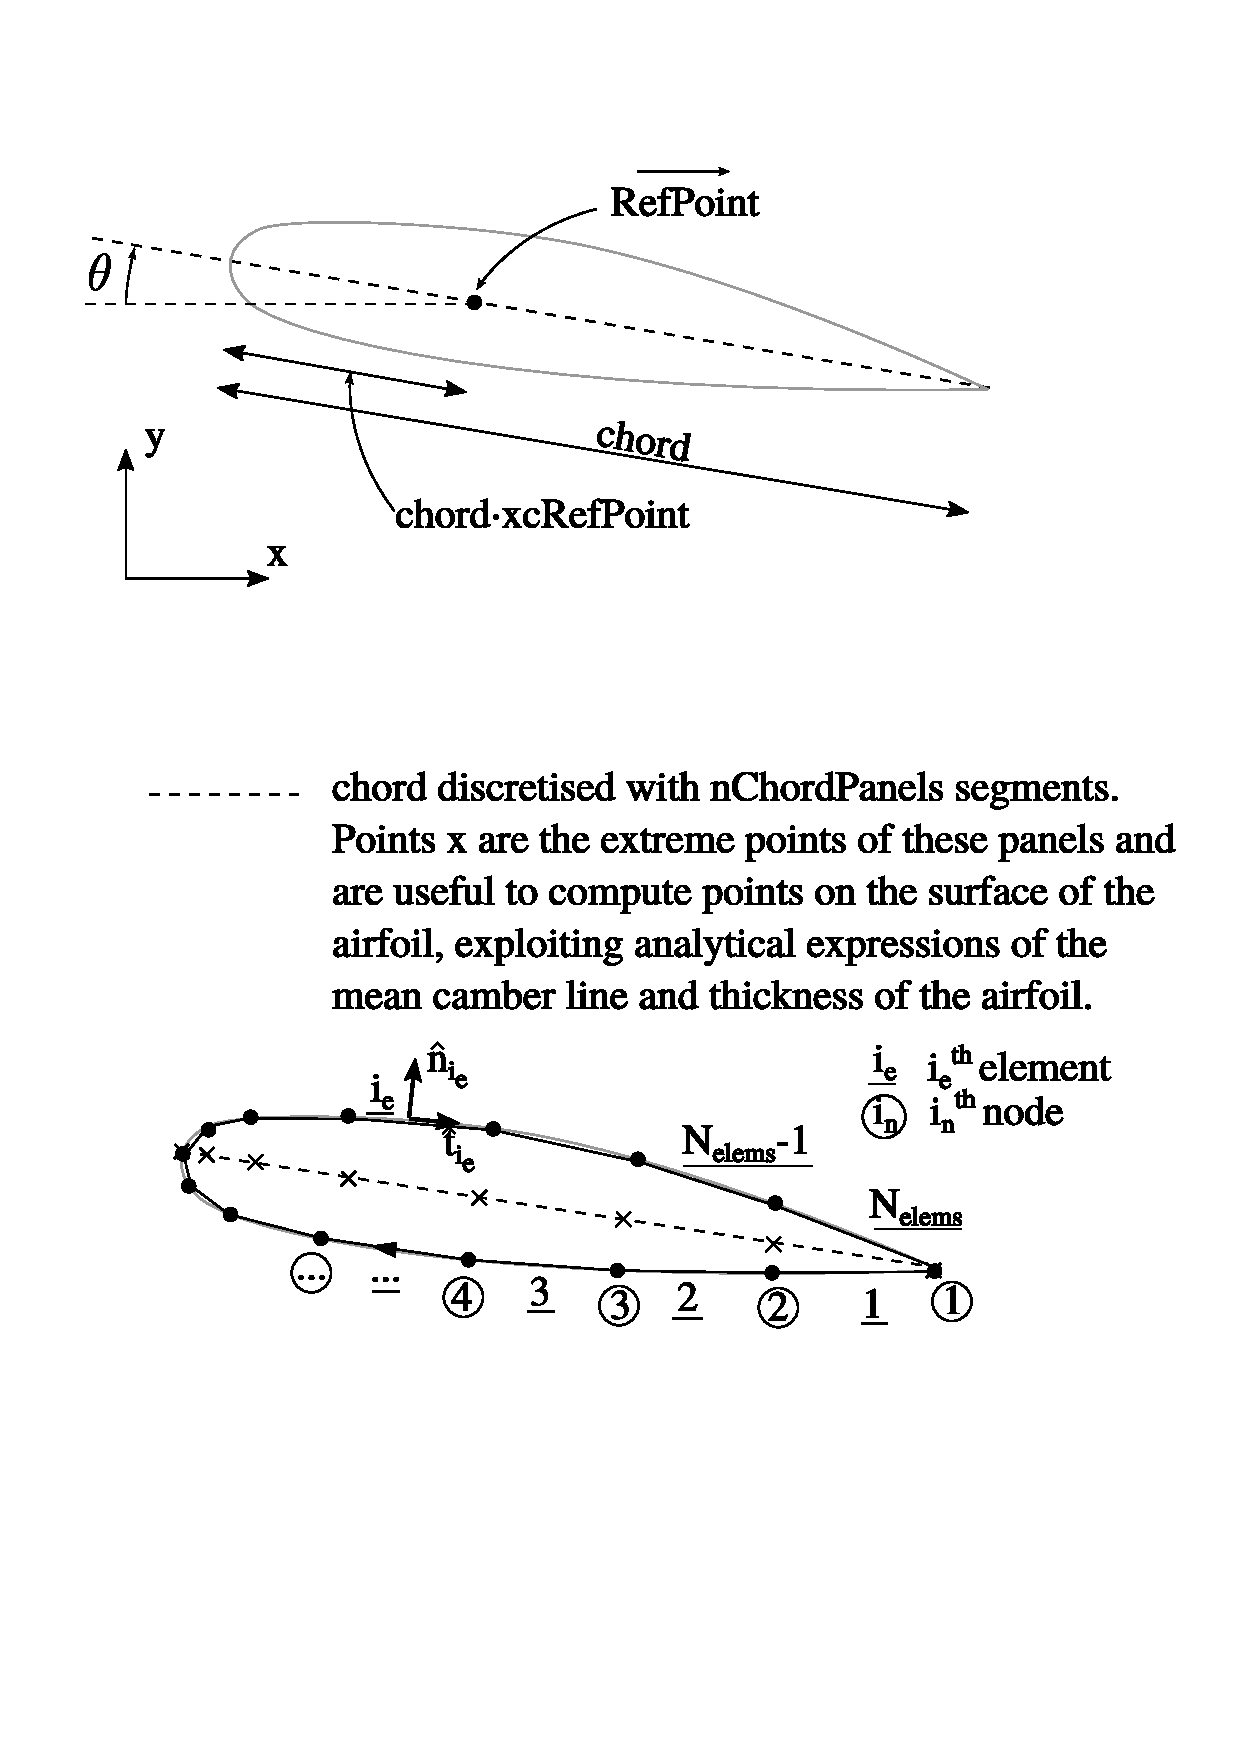
\includepdf[pages=-,pagecommand={},width=\textwidth]{./capitoli/08_aerodinamica/build_geometry.pdf}


